\section{Introdução}
A modelagem do comportamento de partículas em sistemas termodinâmicos macroscópicos encontra como uma das principais dificuldades o valor impraticável de espécies a serem individualmente calculadas, estando na ordem do número de Avogadro. Com isso em vista, passam a ser utilizados métodos estatísticos, uma vez que “da equação de estado só intervêm os valores médios de grandezas microscópicas, tais com a energia cinética média”\cite{Nussenzveig_2014}. Por conta disso, o presente relatório aborda experimentos que exemplificam usos da mecânica estatística para entendimento de propriedades dos gases.

O primeiro tem como enfoque a distribuição normal (ou gaussiana), uma função de densidade de probabilidade muito presente no tratamento estatístico, cuja área da curva entre dois limites indica a chance de encontrar a variável entre esses valores\cite{Gaussiana} e apresenta a forma:
\begin{figure}[H]
    \centering
    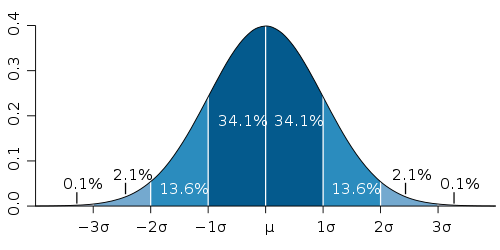
\includegraphics[width=0.5\textwidth]{fig/normal.png}
    \caption{Gráfico de uma função gaussiana. Fonte: \cite{Gaussiana}.}
    \label{fig:grafGaussiana}
\end{figure}

Na experimentação foi analisado um tabuleiro de Galton, criado por Francis Galton para ilustrar como a distribuição normal aproxima-se de uma distribuição binomial. Além disso, mediu-se o preparo de um saco de pipoca no microondas, esperando-se obter uma distribuição gaussiana do número de estouros por tempo.

O segundo experimento envolveu a pressurização do ar em uma garrafa e medição de seu peso, com o objetivo de obter-se a massa e pressão do ar, sendo tal cálculo possível a partir do uso da Lei dos Gases Ideais, uma boa aproximação para a maioria dos gases\cite{Nussenzveig_2014}:
\begin{align}
    PV = nRT
\end{align}
na qual P é a pressão, V o volume, n o número de moles, R a Constante Universal dos Gases e T a temperatura. Portanto, a prática cumpre a finalidade demonstrar a capacidade de medir-se e obter-se valores de grandezas termodinâmicas, bem como o nível de precisão do método utilizado ao comparar-se os resultados com valores de referência.

Por fim, o terceiro ensaio utilizou um equipamento mecânico que simula o comportamento de partículas de um gás em um cilindro de volume variável e energia cinética modulável. Essa experimentação permite a visualização da relação entre as grandezas termodinâmicas, expressa na Lei dos Gases Ideais. Além disso, trata-se de um mecanismo que ilustra a teoria cinética dos gases, sendo esta formulada como um modelo microscópico para o funcionamento da termodinâmica, capaz de modelar diversos fenômenos macroscópicos\cite{Nussenzveig_2014}.
